\chapter{Phase Diversity}
\label{ch:PDThe}

The phase diversity was first implemented by R. A. Gonsalves in 1976 \citep{Gonsalves_1976,Gonsalves_1982} to retrieve the phase of a wavefront coming from a point source. It uses two images, one at the focal plane and another one with a diversity introduced, such as defocus, in order to recover the phase of the wavefront. This chapter introduce the principle on which the phase diversity is based and then describes its implementation with two different algorithms. The first one is an algorithm developed at the ONERA by \citet{mugnier_2006}. The second algorithm presented is the one we developed in the frame of this study, which is based on an analytical approach.

\section{Principle}

\begin{figure}
\begin{center}
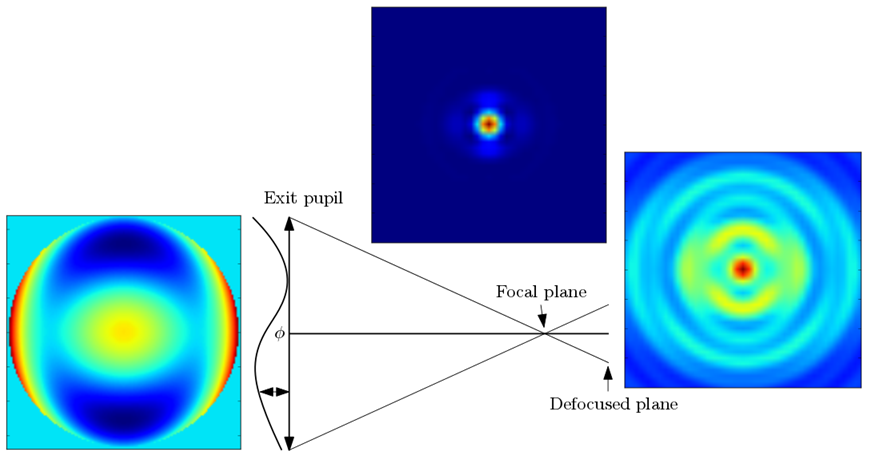
\includegraphics[width=0.8\textwidth,angle=0]{Figures/DiversityPrincipleM}
\decoRule
\caption{Schema of the phase diversity principle. The images from left to right are : the phase arriving on the exit pupil, the focused image and the defocused ($2\pi$) image.}
\label{fig:DiversityPrinciple}
\end{center}
\end{figure}

Unlike Shack-Hartmann wavefront reconstruction, which is a pupil plane technique, the phase diversity uses data acquired at the focal plane. Using the non-linear relation between the phase of the wavefront and the image, 

\begin{equation}
i(x,y) = (h_{optical}\otimes o)(x,y), \ with \ h_{optical}(x,y) = |\left[\mathcal{F}\left\lbrace A(\xi,\eta)e^{j\phi(\xi,\eta)} \right\rbrace\right](x,y)|^2,
\label{eqt:img-hopt}
\end{equation}

one can determine the phase, i.e. the aberrations present in the imaging system, by solving an inverse problem. The major difficulty of this technique is that, as one can see in eqt. \eqref{eqt:img-hopt}, there is not a unique solution to the problem at hand. This indetermination comes from the fact that the available detector can only sense the intensity of the wave, and not the wave itself, which is related to the modulus squared of the complex amplitude as exposed in section \ref{sec:ImSystem}. Thus, $\phi(\xi,\eta)$ and $\phi'(\xi,\eta)=-\phi(-\xi,-\eta)$ give the same PSF.
More specifically by decomposing the phase in its even and odd part and using the autocorrelation properties ($\Gamma_A = \Gamma_{A'}$ with $A'(t) = A*(-t)$), with only one image, one can not determine the sign of the phase even part. This leads to the introduction of a phase diversity to raise the indetermination. The idea is to add a known aberration $\delta\phi$ to the system and to use the two images to retrieve the phase of the wavefront.

The diversity between the two images is introduced for instance by defocusing one of the two images. In this work we will use this diversity, but having a more complex system one could introduce any other even aberration such as an astigmatism, the only requirement is that the diversity introduced must have an even radial and azimuthal order. 

\section{ONERA algorithm}

\section{Analytical algorithm}